
\INEchaptercarta{Caracterización estadística educativa de los matrimonios}{}
\cajita{Matrimonios}{De acuerdo a las estadísticas vitales de 2014, el número de matrimonios, según el período mostrado, mantuvo una tendencia ascendente hasta el 2014, donde este se redujo en un 1.6\% respecto al año anterior.}{Matrimonios}{República de Guatemala, serie histórica, en datos absolutos}{\ \\[0mm]\begin{tikzpicture}[x=1pt,y=1pt]  % Created by tikzDevice version 0.8.1 on 2015-12-11 13:58:54
% !TEX encoding = UTF-8 Unicode
\definecolor{fillColor}{RGB}{255,255,255}
\path[use as bounding box,fill=fillColor,fill opacity=0.00] (0,0) rectangle (289.08,198.74);
\begin{scope}
\path[clip] (  0.00,  0.00) rectangle (289.08,198.74);

\path[] (  0.00,  0.00) rectangle (289.08,198.74);
\end{scope}
\begin{scope}
\path[clip] (  0.00,  0.00) rectangle (289.08,198.74);

\path[] ( 23.32, 17.78) rectangle (280.54,191.48);

\path[] ( 23.32, 44.32) --
	(280.54, 44.32);

\path[] ( 23.32, 81.83) --
	(280.54, 81.83);

\path[] ( 23.32,119.34) --
	(280.54,119.34);

\path[] ( 23.32,156.85) --
	(280.54,156.85);

\path[] ( 23.32, 25.56) --
	(280.54, 25.56);

\path[] ( 23.32, 63.07) --
	(280.54, 63.07);

\path[] ( 23.32,100.58) --
	(280.54,100.58);

\path[] ( 23.32,138.10) --
	(280.54,138.10);

\path[] ( 23.32,175.61) --
	(280.54,175.61);

\path[] ( 53.00, 17.78) --
	( 53.00,191.48);

\path[] (102.46, 17.78) --
	(102.46,191.48);

\path[] (151.93, 17.78) --
	(151.93,191.48);

\path[] (201.40, 17.78) --
	(201.40,191.48);

\path[] (250.86, 17.78) --
	(250.86,191.48);
\definecolor{drawColor}{RGB}{0,0,255}

\path[draw=drawColor,line width= 1.7pt,line join=round] (151.93,183.59) --
	(201.40,177.02) --
	(250.86,174.66);
\definecolor{drawColor}{RGB}{0,0,0}

\node[text=drawColor,anchor=base,inner sep=0pt, outer sep=0pt, scale=  1.01] at (151.93,187.54) {84,253};

\node[text=drawColor,anchor=base west,inner sep=0pt, outer sep=0pt, scale=  1.01] at (201.40,180.97) {80,750};

\node[text=drawColor,anchor=base,inner sep=0pt, outer sep=0pt, scale=  1.01] at (250.86,162.79) {79,496};

\path[draw=drawColor,line width= 0.1pt,line join=round] ( 23.32, 25.67) -- (280.54, 25.67);

\path[] ( 23.32, 17.78) rectangle (280.54,191.48);
\end{scope}
\begin{scope}
\path[clip] (  0.00,  0.00) rectangle (289.08,198.74);

\path[] ( 23.32, 17.78) --
	( 23.32,191.48);
\end{scope}
\begin{scope}
\path[clip] (  0.00,  0.00) rectangle (289.08,198.74);
\definecolor{drawColor}{RGB}{255,255,255}

\node[text=drawColor,text opacity=0.00,anchor=base east,inner sep=0pt, outer sep=0pt, scale=  1.00] at ( 16.20, 21.65) {0};

\node[text=drawColor,text opacity=0.00,anchor=base east,inner sep=0pt, outer sep=0pt, scale=  1.00] at ( 16.20, 59.16) {20000};

\node[text=drawColor,text opacity=0.00,anchor=base east,inner sep=0pt, outer sep=0pt, scale=  1.00] at ( 16.20, 96.68) {40000};

\node[text=drawColor,text opacity=0.00,anchor=base east,inner sep=0pt, outer sep=0pt, scale=  1.00] at ( 16.20,134.19) {60000};

\node[text=drawColor,text opacity=0.00,anchor=base east,inner sep=0pt, outer sep=0pt, scale=  1.00] at ( 16.20,171.70) {80000};
\end{scope}
\begin{scope}
\path[clip] (  0.00,  0.00) rectangle (289.08,198.74);

\path[] ( 19.05, 25.56) --
	( 23.32, 25.56);

\path[] ( 19.05, 63.07) --
	( 23.32, 63.07);

\path[] ( 19.05,100.58) --
	( 23.32,100.58);

\path[] ( 19.05,138.10) --
	( 23.32,138.10);

\path[] ( 19.05,175.61) --
	( 23.32,175.61);
\end{scope}
\begin{scope}
\path[clip] (  0.00,  0.00) rectangle (289.08,198.74);

\path[] ( 23.32, 17.78) --
	(280.54, 17.78);
\end{scope}
\begin{scope}
\path[clip] (  0.00,  0.00) rectangle (289.08,198.74);

\path[] ( 53.00, 13.51) --
	( 53.00, 17.78);

\path[] (102.46, 13.51) --
	(102.46, 17.78);

\path[] (151.93, 13.51) --
	(151.93, 17.78);

\path[] (201.40, 13.51) --
	(201.40, 17.78);

\path[] (250.86, 13.51) --
	(250.86, 17.78);
\end{scope}
\begin{scope}
\path[clip] (  0.00,  0.00) rectangle (289.08,198.74);
\definecolor{drawColor}{RGB}{0,0,0}

\node[text=drawColor,anchor=base,inner sep=0pt, outer sep=0pt, scale=  1.00] at ( 53.00,  2.85) {2010};

\node[text=drawColor,anchor=base,inner sep=0pt, outer sep=0pt, scale=  1.00] at (102.46,  2.85) {2011};

\node[text=drawColor,anchor=base,inner sep=0pt, outer sep=0pt, scale=  1.00] at (151.93,  2.85) {2012};

\node[text=drawColor,anchor=base,inner sep=0pt, outer sep=0pt, scale=  1.00] at (201.40,  2.85) {2013};

\node[text=drawColor,anchor=base,inner sep=0pt, outer sep=0pt, scale=  1.00] at (250.86,  2.85) {2014};
\end{scope}
  \end{tikzpicture}}{Instituto Nacional de Estadística, con datos de estadísticas vitales}
\cajita{Cónyuges sin escolaridad}{Al determinar la proporción de hombres y de mujeres que contrajeron matrimonio en el período 2011-2014, que no tenían ningún nivel de escolaridad, se observa que la tendencia ha sido descendiente para ambos, aunque tuvo un aumento en el 2014 de 1.9 puntos porcentuales para las mujeres y de 0.8 para los hombres respecto al 2013.}{Proporción de hombres y de mujeres sin ningún nivel de escolaridad que contrajeron matrimonio }{República de Guatemala, serie histórica, en proporción}{\ \\[0mm]\begin{tikzpicture}[x=1pt,y=1pt]  % Created by tikzDevice version 0.10.1 on 2016-02-29 14:48:27
% !TEX encoding = UTF-8 Unicode
\definecolor{fillColor}{RGB}{255,255,255}
\path[use as bounding box,fill=fillColor,fill opacity=0.00] (0,0) rectangle (289.08,198.74);
\begin{scope}
\path[clip] (  0.00,  0.00) rectangle (289.08,198.74);

\path[] (  0.00,  0.00) rectangle (289.08,198.74);
\end{scope}
\begin{scope}
\path[clip] (  0.00,  0.00) rectangle (289.08,198.74);

\path[] (  0.00, 18.46) rectangle (289.08,172.85);

\path[] ( 33.36, 18.46) --
	( 33.36,172.85);

\path[] ( 88.95, 18.46) --
	( 88.95,172.85);

\path[] (144.54, 18.46) --
	(144.54,172.85);

\path[] (200.13, 18.46) --
	(200.13,172.85);

\path[] (255.72, 18.46) --
	(255.72,172.85);
\definecolor{drawColor}{RGB}{0,0,255}
\definecolor{fillColor}{RGB}{0,0,255}

\path[draw=drawColor,line width= 0.6pt,line join=round,fill=fillColor] ( 13.20, 18.46) rectangle ( 28.49,172.85);
\definecolor{drawColor}{RGB}{157,187,255}
\definecolor{fillColor}{RGB}{157,187,255}

\path[draw=drawColor,line width= 0.6pt,line join=round,fill=fillColor] ( 38.22, 18.46) rectangle ( 53.51,150.59);
\definecolor{drawColor}{RGB}{0,0,255}
\definecolor{fillColor}{RGB}{0,0,255}

\path[draw=drawColor,line width= 0.6pt,line join=round,fill=fillColor] ( 68.80, 18.46) rectangle ( 84.08,163.21);
\definecolor{drawColor}{RGB}{157,187,255}
\definecolor{fillColor}{RGB}{157,187,255}

\path[draw=drawColor,line width= 0.6pt,line join=round,fill=fillColor] ( 93.81, 18.46) rectangle (109.10,131.52);
\definecolor{drawColor}{RGB}{0,0,255}
\definecolor{fillColor}{RGB}{0,0,255}

\path[draw=drawColor,line width= 0.6pt,line join=round,fill=fillColor] (124.39, 18.46) rectangle (139.68,154.24);
\definecolor{drawColor}{RGB}{157,187,255}
\definecolor{fillColor}{RGB}{157,187,255}

\path[draw=drawColor,line width= 0.6pt,line join=round,fill=fillColor] (149.40, 18.46) rectangle (164.69,113.28);
\definecolor{drawColor}{RGB}{0,0,255}
\definecolor{fillColor}{RGB}{0,0,255}

\path[draw=drawColor,line width= 0.6pt,line join=round,fill=fillColor] (179.98, 18.46) rectangle (195.27,115.45);
\definecolor{drawColor}{RGB}{157,187,255}
\definecolor{fillColor}{RGB}{157,187,255}

\path[draw=drawColor,line width= 0.6pt,line join=round,fill=fillColor] (205.00, 18.46) rectangle (220.28, 75.93);
\definecolor{drawColor}{RGB}{0,0,255}
\definecolor{fillColor}{RGB}{0,0,255}

\path[draw=drawColor,line width= 0.6pt,line join=round,fill=fillColor] (235.57, 18.46) rectangle (250.86,123.90);
\definecolor{drawColor}{RGB}{157,187,255}
\definecolor{fillColor}{RGB}{157,187,255}

\path[draw=drawColor,line width= 0.6pt,line join=round,fill=fillColor] (260.59, 18.46) rectangle (275.88, 79.74);
\definecolor{drawColor}{RGB}{0,0,0}

\path[draw=drawColor,line width= 0.6pt,line join=round] (  0.00, 18.46) -- (289.08, 18.46);

\node[text=drawColor,anchor=base,inner sep=0pt, outer sep=0pt, scale=  0.83] at ( 20.85,176.08) {34.0};

\node[text=drawColor,anchor=base,inner sep=0pt, outer sep=0pt, scale=  0.83] at ( 45.86,153.83) {29.1};

\node[text=drawColor,anchor=base,inner sep=0pt, outer sep=0pt, scale=  0.83] at ( 76.44,166.44) {31.9};

\node[text=drawColor,anchor=base,inner sep=0pt, outer sep=0pt, scale=  0.83] at (101.46,134.75) {24.9};

\node[text=drawColor,anchor=base,inner sep=0pt, outer sep=0pt, scale=  0.83] at (132.03,157.47) {29.9};

\node[text=drawColor,anchor=base,inner sep=0pt, outer sep=0pt, scale=  0.83] at (157.05,116.51) {20.9};

\node[text=drawColor,anchor=base,inner sep=0pt, outer sep=0pt, scale=  0.83] at (187.62,118.68) {21.4};

\node[text=drawColor,anchor=base,inner sep=0pt, outer sep=0pt, scale=  0.83] at (212.64, 79.16) {12.7};

\node[text=drawColor,anchor=base,inner sep=0pt, outer sep=0pt, scale=  0.83] at (243.22,127.14) {23.2};

\node[text=drawColor,anchor=base,inner sep=0pt, outer sep=0pt, scale=  0.83] at (268.23, 82.97) {13.5};

\path[] (  0.00, 18.46) rectangle (289.08,172.85);
\end{scope}
\begin{scope}
\path[clip] (  0.00,  0.00) rectangle (289.08,198.74);

\path[] (  0.00, 18.46) --
	(289.08, 18.46);
\end{scope}
\begin{scope}
\path[clip] (  0.00,  0.00) rectangle (289.08,198.74);

\path[] ( 33.36, 15.71) --
	( 33.36, 18.46);

\path[] ( 88.95, 15.71) --
	( 88.95, 18.46);

\path[] (144.54, 15.71) --
	(144.54, 18.46);

\path[] (200.13, 15.71) --
	(200.13, 18.46);

\path[] (255.72, 15.71) --
	(255.72, 18.46);
\end{scope}
\begin{scope}
\path[clip] (  0.00,  0.00) rectangle (289.08,198.74);
\definecolor{drawColor}{RGB}{0,0,0}

\node[text=drawColor,anchor=base,inner sep=0pt, outer sep=0pt, scale=  1.00] at ( 33.36,  5.69) {2010};

\node[text=drawColor,anchor=base,inner sep=0pt, outer sep=0pt, scale=  1.00] at ( 88.95,  5.69) {2011};

\node[text=drawColor,anchor=base,inner sep=0pt, outer sep=0pt, scale=  1.00] at (144.54,  5.69) {2012};

\node[text=drawColor,anchor=base,inner sep=0pt, outer sep=0pt, scale=  1.00] at (200.13,  5.69) {2013};

\node[text=drawColor,anchor=base,inner sep=0pt, outer sep=0pt, scale=  1.00] at (255.72,  5.69) {2014};
\end{scope}
\begin{scope}
\path[clip] (  0.00,  0.00) rectangle (289.08,198.74);
\coordinate (apoyo) at (59.42,189.21);
\coordinate (longitudFicticia) at (7.11,9.53);
\coordinate (longitud) at (7.11,7.11);
\coordinate (desX) at (135.34,0);
\coordinate (desY) at (0,1.21);
\definecolor[named]{ct1}{HTML}{
0000FF
}
\definecolor[named]{ct2}{HTML}{
9DBBFF
}
\definecolor[named]{ctb1}{HTML}{
0000FF
}
\definecolor[named]{ctb2}{HTML}{
9DBBFF
}
\path [fill=none] (apoyo) rectangle ($(apoyo)+(longitudFicticia)$)
node [xshift=0.3cm,inner sep=0pt, outer sep=0pt,midway,right,scale = 0.9]{Mujer};
\draw [color = ctb1,fill=ct1] ( $(apoyo)  + (desY) $) rectangle ($(apoyo)+ (desY) +(longitud)$);
\path [fill=none] ($(apoyo)+(desX)$) rectangle ($(apoyo)+(desX)+(longitudFicticia)$)
node [xshift=0.3cm,inner sep=0pt, outer sep=0pt,midway,right,scale = 0.9]{Hombre};
\draw [color = ctb2 ,fill=ct2] ( $(apoyo)  + (desY) + (desX) $) rectangle ($(apoyo)+ (desY)+ (desX) +(longitud)$);
\end{scope}
  \end{tikzpicture}}{Instituto Nacional de Estadística, con datos de estadísticas vitales}
\cajita{Cónyuges universitarios}{En cuanto a las personas que contrajeron matrimonio teniendo algún estudio a nivel universitario hasta un posgrado, se observa que esta proporción tienen una tendencia ascendente, siendo de 3.7 mujeres con estudio universitario por cada 100 que se casaron y de los hombres de 4.5.\textollamada{Desde el 2012 en el registro se hace distinción entre nivel universitario y nivel de posgrado. Las proporciones mostradas para 2012 y 2013 incluye a ambos grupos.}}{Proporción de hombres y de mujeres estudios universitarios que contrajeron matrimonio }{República de Guatemala, serie histórica, en proporción}{\ \\[0mm]\begin{tikzpicture}[x=1pt,y=1pt]  % Created by tikzDevice version 0.10.1 on 2016-02-29 14:49:45
% !TEX encoding = UTF-8 Unicode
\definecolor{fillColor}{RGB}{255,255,255}
\path[use as bounding box,fill=fillColor,fill opacity=0.00] (0,0) rectangle (289.08,198.74);
\begin{scope}
\path[clip] (  0.00,  0.00) rectangle (289.08,198.74);

\path[] (  0.00,  0.00) rectangle (289.08,198.74);
\end{scope}
\begin{scope}
\path[clip] (  0.00,  0.00) rectangle (289.08,198.74);

\path[] (  0.00, 18.46) rectangle (289.08,172.85);

\path[] ( 33.36, 18.46) --
	( 33.36,172.85);

\path[] ( 88.95, 18.46) --
	( 88.95,172.85);

\path[] (144.54, 18.46) --
	(144.54,172.85);

\path[] (200.13, 18.46) --
	(200.13,172.85);

\path[] (255.72, 18.46) --
	(255.72,172.85);
\definecolor{drawColor}{RGB}{0,0,255}
\definecolor{fillColor}{RGB}{0,0,255}

\path[draw=drawColor,line width= 0.6pt,line join=round,fill=fillColor] ( 13.20, 18.46) rectangle ( 28.49, 70.79);
\definecolor{drawColor}{RGB}{157,187,255}
\definecolor{fillColor}{RGB}{157,187,255}

\path[draw=drawColor,line width= 0.6pt,line join=round,fill=fillColor] ( 38.22, 18.46) rectangle ( 53.51, 80.22);
\definecolor{drawColor}{RGB}{0,0,255}
\definecolor{fillColor}{RGB}{0,0,255}

\path[draw=drawColor,line width= 0.6pt,line join=round,fill=fillColor] ( 68.80, 18.46) rectangle ( 84.08, 97.55);
\definecolor{drawColor}{RGB}{157,187,255}
\definecolor{fillColor}{RGB}{157,187,255}

\path[draw=drawColor,line width= 0.6pt,line join=round,fill=fillColor] ( 93.81, 18.46) rectangle (109.10,114.33);
\definecolor{drawColor}{RGB}{0,0,255}
\definecolor{fillColor}{RGB}{0,0,255}

\path[draw=drawColor,line width= 0.6pt,line join=round,fill=fillColor] (124.39, 18.46) rectangle (139.68,119.73);
\definecolor{drawColor}{RGB}{157,187,255}
\definecolor{fillColor}{RGB}{157,187,255}

\path[draw=drawColor,line width= 0.6pt,line join=round,fill=fillColor] (149.40, 18.46) rectangle (164.69,136.96);
\definecolor{drawColor}{RGB}{0,0,255}
\definecolor{fillColor}{RGB}{0,0,255}

\path[draw=drawColor,line width= 0.6pt,line join=round,fill=fillColor] (179.98, 18.46) rectangle (195.27,141.97);
\definecolor{drawColor}{RGB}{157,187,255}
\definecolor{fillColor}{RGB}{157,187,255}

\path[draw=drawColor,line width= 0.6pt,line join=round,fill=fillColor] (205.00, 18.46) rectangle (220.28,167.55);
\definecolor{drawColor}{RGB}{0,0,255}
\definecolor{fillColor}{RGB}{0,0,255}

\path[draw=drawColor,line width= 0.6pt,line join=round,fill=fillColor] (235.57, 18.46) rectangle (250.86,143.23);
\definecolor{drawColor}{RGB}{157,187,255}
\definecolor{fillColor}{RGB}{157,187,255}

\path[draw=drawColor,line width= 0.6pt,line join=round,fill=fillColor] (260.59, 18.46) rectangle (275.88,172.85);
\definecolor{drawColor}{RGB}{0,0,0}

\path[draw=drawColor,line width= 0.6pt,line join=round] (  0.00, 18.46) -- (289.08, 18.46);

\node[text=drawColor,anchor=base,inner sep=0pt, outer sep=0pt, scale=  0.83] at ( 20.85, 74.03) {1.5};

\node[text=drawColor,anchor=base,inner sep=0pt, outer sep=0pt, scale=  0.83] at ( 45.86, 83.46) {1.8};

\node[text=drawColor,anchor=base,inner sep=0pt, outer sep=0pt, scale=  0.83] at ( 76.44,100.79) {2.3};

\node[text=drawColor,anchor=base,inner sep=0pt, outer sep=0pt, scale=  0.83] at (101.46,117.56) {2.8};

\node[text=drawColor,anchor=base,inner sep=0pt, outer sep=0pt, scale=  0.83] at (132.03,122.97) {2.9};

\node[text=drawColor,anchor=base,inner sep=0pt, outer sep=0pt, scale=  0.83] at (157.05,140.20) {3.4};

\node[text=drawColor,anchor=base,inner sep=0pt, outer sep=0pt, scale=  0.83] at (187.62,145.21) {3.6};

\node[text=drawColor,anchor=base,inner sep=0pt, outer sep=0pt, scale=  0.83] at (212.64,170.78) {4.3};

\node[text=drawColor,anchor=base,inner sep=0pt, outer sep=0pt, scale=  0.83] at (243.22,146.46) {3.6};

\node[text=drawColor,anchor=base,inner sep=0pt, outer sep=0pt, scale=  0.83] at (268.23,176.08) {4.5};

\path[] (  0.00, 18.46) rectangle (289.08,172.85);
\end{scope}
\begin{scope}
\path[clip] (  0.00,  0.00) rectangle (289.08,198.74);

\path[] (  0.00, 18.46) --
	(289.08, 18.46);
\end{scope}
\begin{scope}
\path[clip] (  0.00,  0.00) rectangle (289.08,198.74);

\path[] ( 33.36, 15.71) --
	( 33.36, 18.46);

\path[] ( 88.95, 15.71) --
	( 88.95, 18.46);

\path[] (144.54, 15.71) --
	(144.54, 18.46);

\path[] (200.13, 15.71) --
	(200.13, 18.46);

\path[] (255.72, 15.71) --
	(255.72, 18.46);
\end{scope}
\begin{scope}
\path[clip] (  0.00,  0.00) rectangle (289.08,198.74);
\definecolor{drawColor}{RGB}{0,0,0}

\node[text=drawColor,anchor=base,inner sep=0pt, outer sep=0pt, scale=  1.00] at ( 33.36,  5.69) {2010};

\node[text=drawColor,anchor=base,inner sep=0pt, outer sep=0pt, scale=  1.00] at ( 88.95,  5.69) {2011};

\node[text=drawColor,anchor=base,inner sep=0pt, outer sep=0pt, scale=  1.00] at (144.54,  5.69) {2012};

\node[text=drawColor,anchor=base,inner sep=0pt, outer sep=0pt, scale=  1.00] at (200.13,  5.69) {2013};

\node[text=drawColor,anchor=base,inner sep=0pt, outer sep=0pt, scale=  1.00] at (255.72,  5.69) {2014};
\end{scope}
\begin{scope}
\path[clip] (  0.00,  0.00) rectangle (289.08,198.74);
\coordinate (apoyo) at (59.42,189.21);
\coordinate (longitudFicticia) at (7.11,9.53);
\coordinate (longitud) at (7.11,7.11);
\coordinate (desX) at (135.34,0);
\coordinate (desY) at (0,1.21);
\definecolor[named]{ct1}{HTML}{
0000FF
}
\definecolor[named]{ct2}{HTML}{
9DBBFF
}
\definecolor[named]{ctb1}{HTML}{
0000FF
}
\definecolor[named]{ctb2}{HTML}{
9DBBFF
}
\path [fill=none] (apoyo) rectangle ($(apoyo)+(longitudFicticia)$)
node [xshift=0.3cm,inner sep=0pt, outer sep=0pt,midway,right,scale = 0.9]{Mujer};
\draw [color = ctb1,fill=ct1] ( $(apoyo)  + (desY) $) rectangle ($(apoyo)+ (desY) +(longitud)$);
\path [fill=none] ($(apoyo)+(desX)$) rectangle ($(apoyo)+(desX)+(longitudFicticia)$)
node [xshift=0.3cm,inner sep=0pt, outer sep=0pt,midway,right,scale = 0.9]{Hombre};
\draw [color = ctb2 ,fill=ct2] ( $(apoyo)  + (desY) + (desX) $) rectangle ($(apoyo)+ (desY)+ (desX) +(longitud)$);
\end{scope}
  \end{tikzpicture}}{Instituto Nacional de Estadística, con datos de estadísticas vitales}
\cajita{Mujeres sin escolaridad según nivel escolar del hombre}{Al tomar al grupo de mujeres que contrajeron matrimonio en el 2014 que no tenían ningún nivel de escolaridad y desagregarlo según el nivel de estudio del hombre contrayente, se observa que principalmente el esposo tiene algún grado de educación primaria.}{Distribución de mujeres sin escolaridad que contrajeron matrimonio según la escolaridad del hombre}{República de Guatemala, año 2014, en proporción}{\ \\[0mm]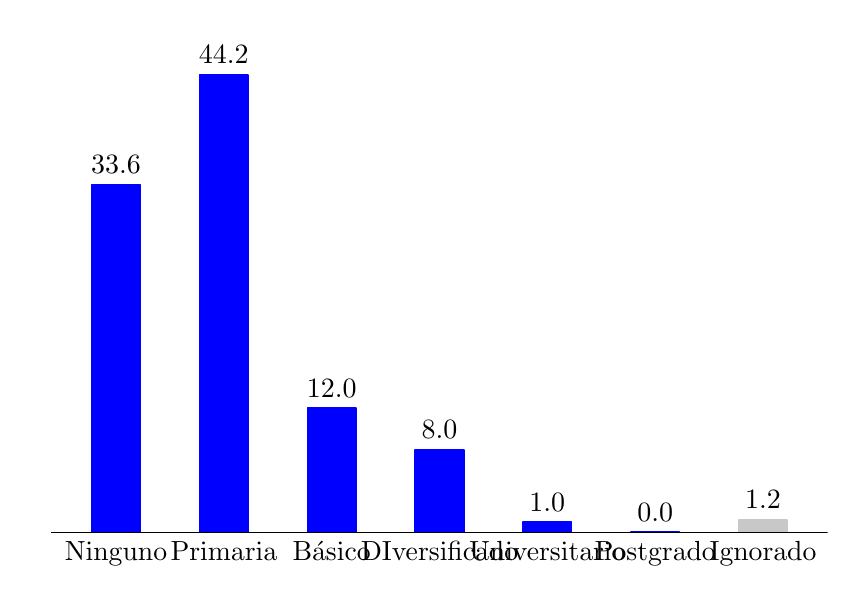
\begin{tikzpicture}[x=1pt,y=1pt]  % Created by tikzDevice version 0.8.1 on 2015-12-11 13:59:06
% !TEX encoding = UTF-8 Unicode
\definecolor{fillColor}{RGB}{255,255,255}
\path[use as bounding box,fill=fillColor,fill opacity=0.00] (0,0) rectangle (289.08,198.74);
\begin{scope}
\path[clip] (  0.00,  0.00) rectangle (289.08,198.74);

\path[] (  0.00,  0.00) rectangle (289.08,198.74);
\end{scope}
\begin{scope}
\path[clip] (  0.00,  0.00) rectangle (289.08,198.74);

\path[] (  8.54, 16.35) rectangle (289.08,181.67);

\path[] ( 31.91, 16.35) --
	( 31.91,181.67);

\path[] ( 70.88, 16.35) --
	( 70.88,181.67);

\path[] (109.84, 16.35) --
	(109.84,181.67);

\path[] (148.81, 16.35) --
	(148.81,181.67);

\path[] (187.77, 16.35) --
	(187.77,181.67);

\path[] (226.74, 16.35) --
	(226.74,181.67);

\path[] (265.70, 16.35) --
	(265.70,181.67);
\definecolor{drawColor}{RGB}{0,0,255}
\definecolor{fillColor}{RGB}{0,0,255}

\path[draw=drawColor,line width= 0.6pt,line join=round,fill=fillColor] ( 23.15, 16.35) rectangle ( 40.68,142.05);

\path[draw=drawColor,line width= 0.6pt,line join=round,fill=fillColor] ( 62.11, 16.35) rectangle ( 79.65,181.67);

\path[draw=drawColor,line width= 0.6pt,line join=round,fill=fillColor] (101.08, 16.35) rectangle (118.61, 61.32);

\path[draw=drawColor,line width= 0.6pt,line join=round,fill=fillColor] (140.04, 16.35) rectangle (157.57, 46.16);

\path[draw=drawColor,line width= 0.6pt,line join=round,fill=fillColor] (179.01, 16.35) rectangle (196.54, 20.10);

\path[draw=drawColor,line width= 0.6pt,line join=round,fill=fillColor] (217.97, 16.35) rectangle (235.50, 16.47);
\definecolor{drawColor}{RGB}{200,200,200}
\definecolor{fillColor}{RGB}{200,200,200}

\path[draw=drawColor,line width= 0.6pt,line join=round,fill=fillColor] (256.93, 16.35) rectangle (274.47, 20.89);
\definecolor{drawColor}{RGB}{0,0,0}

\path[draw=drawColor,line width= 0.1pt,line join=round] (  8.54, 16.35) -- (289.08, 16.35);

\node[text=drawColor,anchor=base,inner sep=0pt, outer sep=0pt, scale=  1.01] at ( 31.91,146.01) {33.6};

\node[text=drawColor,anchor=base,inner sep=0pt, outer sep=0pt, scale=  1.01] at ( 70.88,185.63) {44.2};

\node[text=drawColor,anchor=base,inner sep=0pt, outer sep=0pt, scale=  1.01] at (109.84, 65.28) {12.0};

\node[text=drawColor,anchor=base,inner sep=0pt, outer sep=0pt, scale=  1.01] at (148.81, 50.12) {8.0};

\node[text=drawColor,anchor=base,inner sep=0pt, outer sep=0pt, scale=  1.01] at (187.77, 24.06) {1.0};

\node[text=drawColor,anchor=base,inner sep=0pt, outer sep=0pt, scale=  1.01] at (226.74, 20.43) {0.0};

\node[text=drawColor,anchor=base,inner sep=0pt, outer sep=0pt, scale=  1.01] at (265.70, 24.85) {1.2};

\path[] (  8.54, 16.35) rectangle (289.08,181.67);
\end{scope}
\begin{scope}
\path[clip] (  0.00,  0.00) rectangle (289.08,198.74);

\path[] (  8.54, 16.35) --
	(  8.54,181.67);
\end{scope}
\begin{scope}
\path[clip] (  0.00,  0.00) rectangle (289.08,198.74);

\path[] (  8.54, 16.35) --
	(289.08, 16.35);
\end{scope}
\begin{scope}
\path[clip] (  0.00,  0.00) rectangle (289.08,198.74);

\path[] ( 31.91, 12.08) --
	( 31.91, 16.35);

\path[] ( 70.88, 12.08) --
	( 70.88, 16.35);

\path[] (109.84, 12.08) --
	(109.84, 16.35);

\path[] (148.81, 12.08) --
	(148.81, 16.35);

\path[] (187.77, 12.08) --
	(187.77, 16.35);

\path[] (226.74, 12.08) --
	(226.74, 16.35);

\path[] (265.70, 12.08) --
	(265.70, 16.35);
\end{scope}
\begin{scope}
\path[clip] (  0.00,  0.00) rectangle (289.08,198.74);
\definecolor{drawColor}{RGB}{0,0,0}

\node[text=drawColor,anchor=base,inner sep=0pt, outer sep=0pt, scale=  1.00] at ( 31.91,  6.04) {Ninguno};

\node[text=drawColor,anchor=base,inner sep=0pt, outer sep=0pt, scale=  1.00] at ( 70.88,  6.04) {Primaria};

\node[text=drawColor,anchor=base,inner sep=0pt, outer sep=0pt, scale=  1.00] at (109.84,  6.04) {Básico};

\node[text=drawColor,anchor=base,inner sep=0pt, outer sep=0pt, scale=  1.00] at (148.81,  6.04) {DIversificado};

\node[text=drawColor,anchor=base,inner sep=0pt, outer sep=0pt, scale=  1.00] at (187.77,  6.04) {Universitario};

\node[text=drawColor,anchor=base,inner sep=0pt, outer sep=0pt, scale=  1.00] at (226.74,  6.04) {Postgrado};

\node[text=drawColor,anchor=base,inner sep=0pt, outer sep=0pt, scale=  1.00] at (265.70,  6.04) {Ignorado};
\end{scope}
  \end{tikzpicture}}{Instituto Nacional de Estadística, con datos de estadísticas vitales}
\cajita{Mujeres universitarias según nivel escolar del hombre}{La gráfica muestra el nivel escolar del hombre contrajo matrimonio con una mujer con nivel universitario. Se observa que mayormente, el esposo tiene algún grado de educación diversificada. En el 39.5\% de los casos tanto la mujer como el hombre tienen nivel universitario.\textollamada{Debido a que la base de datos de 2014 distingue entre nivel universitario y de posgrado, la distribución mostrada incluye únicamente a las mujeres con escolaridad universitaria y no a las de posgrado.}}{Distribución de mujeres con estudios universitarios  que contrajeron matrimonio según la escolaridad del hombre}{República de Guatemala, año 2014, en proporción}{\ \\[0mm]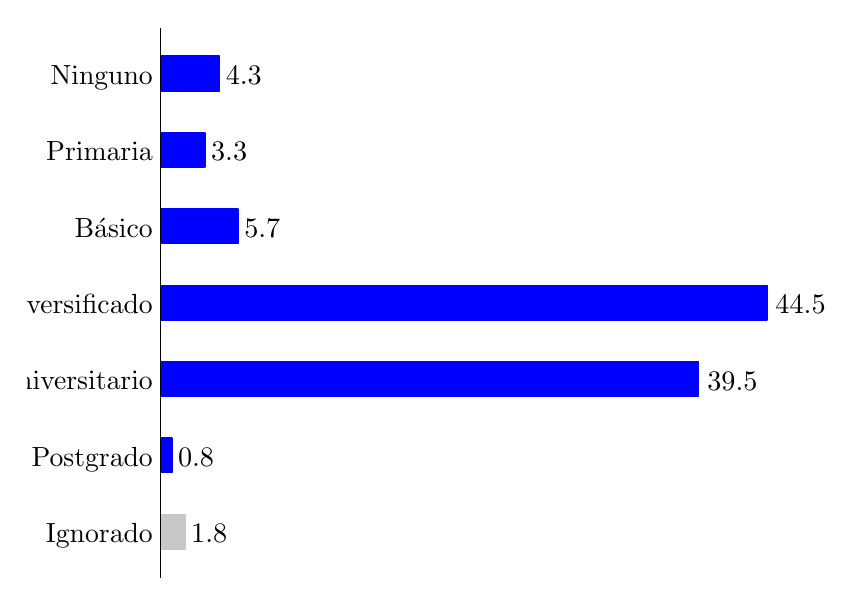
\begin{tikzpicture}[x=1pt,y=1pt]  % Created by tikzDevice version 0.10.1 on 2016-02-29 14:51:35
% !TEX encoding = UTF-8 Unicode
\definecolor{fillColor}{RGB}{255,255,255}
\path[use as bounding box,fill=fillColor,fill opacity=0.00] (0,0) rectangle (289.08,198.74);
\begin{scope}
\path[clip] (  0.00,  0.00) rectangle (289.08,198.74);

\path[] (  0.00,  0.00) rectangle (289.08,198.74);
\end{scope}
\begin{scope}
\path[clip] (  0.00,  0.00) rectangle (289.08,198.74);

\path[] ( 47.97,  0.00) rectangle (267.09,198.74);

\path[] ( 47.97, 16.56) --
	(267.09, 16.56);

\path[] ( 47.97, 44.16) --
	(267.09, 44.16);

\path[] ( 47.97, 71.77) --
	(267.09, 71.77);

\path[] ( 47.97, 99.37) --
	(267.09, 99.37);

\path[] ( 47.97,126.97) --
	(267.09,126.97);

\path[] ( 47.97,154.58) --
	(267.09,154.58);

\path[] ( 47.97,182.18) --
	(267.09,182.18);
\definecolor{drawColor}{RGB}{200,200,200}
\definecolor{fillColor}{RGB}{200,200,200}

\path[draw=drawColor,line width= 0.6pt,line join=round,fill=fillColor] ( 47.97, 10.35) rectangle ( 56.87, 22.77);
\definecolor{drawColor}{RGB}{0,0,255}
\definecolor{fillColor}{RGB}{0,0,255}

\path[draw=drawColor,line width= 0.6pt,line join=round,fill=fillColor] ( 47.97, 37.95) rectangle ( 52.08, 50.38);

\path[draw=drawColor,line width= 0.6pt,line join=round,fill=fillColor] ( 47.97, 65.56) rectangle (242.45, 77.98);

\path[draw=drawColor,line width= 0.6pt,line join=round,fill=fillColor] ( 47.97, 93.16) rectangle (267.09,105.58);

\path[draw=drawColor,line width= 0.6pt,line join=round,fill=fillColor] ( 47.97,120.76) rectangle ( 76.02,133.19);

\path[draw=drawColor,line width= 0.6pt,line join=round,fill=fillColor] ( 47.97,148.37) rectangle ( 64.05,160.79);

\path[draw=drawColor,line width= 0.6pt,line join=round,fill=fillColor] ( 47.97,175.97) rectangle ( 69.35,188.39);
\definecolor{drawColor}{RGB}{0,0,0}

\path[draw=drawColor,line width= 0.1pt,line join=round] ( 47.97,  0.00) -- ( 47.97,198.74);

\node[text=drawColor,anchor=base west,inner sep=0pt, outer sep=0pt, scale=  1.02] at ( 59.10, 12.59) {1.8};

\node[text=drawColor,anchor=base west,inner sep=0pt, outer sep=0pt, scale=  1.02] at ( 54.32, 40.19) {0.8};

\node[text=drawColor,anchor=base west,inner sep=0pt, outer sep=0pt, scale=  1.02] at (245.58, 67.80) {39.5};

\node[text=drawColor,anchor=base west,inner sep=0pt, outer sep=0pt, scale=  1.02] at (270.21, 95.40) {44.5};

\node[text=drawColor,anchor=base west,inner sep=0pt, outer sep=0pt, scale=  1.02] at ( 78.26,123.00) {5.7};

\node[text=drawColor,anchor=base west,inner sep=0pt, outer sep=0pt, scale=  1.02] at ( 66.29,150.61) {3.3};

\node[text=drawColor,anchor=base west,inner sep=0pt, outer sep=0pt, scale=  1.02] at ( 71.59,178.21) {4.3};

\path[] ( 47.97,  0.00) rectangle (267.09,198.74);
\end{scope}
\begin{scope}
\path[clip] (  0.00,  0.00) rectangle (289.08,198.74);

\path[] ( 47.97,  0.00) --
	( 47.97,198.74);
\end{scope}
\begin{scope}
\path[clip] (  0.00,  0.00) rectangle (289.08,198.74);
\definecolor{drawColor}{RGB}{0,0,0}

\node[text=drawColor,anchor=base east,inner sep=0pt, outer sep=0pt, scale=  1.00] at ( 45.22, 12.65) {Ignorado};

\node[text=drawColor,anchor=base east,inner sep=0pt, outer sep=0pt, scale=  1.00] at ( 45.22, 40.26) {Postgrado};

\node[text=drawColor,anchor=base east,inner sep=0pt, outer sep=0pt, scale=  1.00] at ( 45.22, 67.86) {Universitario};

\node[text=drawColor,anchor=base east,inner sep=0pt, outer sep=0pt, scale=  1.00] at ( 45.22, 95.46) {DIversificado};

\node[text=drawColor,anchor=base east,inner sep=0pt, outer sep=0pt, scale=  1.00] at ( 45.22,123.07) {Básico};

\node[text=drawColor,anchor=base east,inner sep=0pt, outer sep=0pt, scale=  1.00] at ( 45.22,150.67) {Primaria};

\node[text=drawColor,anchor=base east,inner sep=0pt, outer sep=0pt, scale=  1.00] at ( 45.22,178.27) {Ninguno};
\end{scope}
\begin{scope}
\path[clip] (  0.00,  0.00) rectangle (289.08,198.74);

\path[] ( 45.22, 16.56) --
	( 47.97, 16.56);

\path[] ( 45.22, 44.16) --
	( 47.97, 44.16);

\path[] ( 45.22, 71.77) --
	( 47.97, 71.77);

\path[] ( 45.22, 99.37) --
	( 47.97, 99.37);

\path[] ( 45.22,126.97) --
	( 47.97,126.97);

\path[] ( 45.22,154.58) --
	( 47.97,154.58);

\path[] ( 45.22,182.18) --
	( 47.97,182.18);
\end{scope}
  \end{tikzpicture}}{Instituto Nacional de Estadística, con datos de estadísticas vitales}
\cajita{Edad según nivel de escolaridad}{Se distingue que la edad mediana de los contrayentes, según el nivel de escolaridad, es generalmente mayor entre los hombres que las mujeres, la excepción se observa en el nivel posgrado.}{Edad mediana de los hombres y las mujeres que contraen matrimonio según nivel de escolaridad }{República de Guatemala, año 2014, en años}{\ \\[0mm]\begin{tikzpicture}[x=1pt,y=1pt]  % Created by tikzDevice version 0.10.1 on 2016-02-29 14:51:58
% !TEX encoding = UTF-8 Unicode
\definecolor{fillColor}{RGB}{255,255,255}
\path[use as bounding box,fill=fillColor,fill opacity=0.00] (0,0) rectangle (289.08,198.74);
\begin{scope}
\path[clip] (  0.00,  0.00) rectangle (289.08,198.74);

\path[] (  0.00,  0.00) rectangle (289.08,198.74);
\end{scope}
\begin{scope}
\path[clip] (  0.00,  0.00) rectangle (289.08,198.74);

\path[] (  0.00, 55.86) rectangle (289.08,172.85);

\path[] ( 27.98, 55.86) --
	( 27.98,172.85);

\path[] ( 74.60, 55.86) --
	( 74.60,172.85);

\path[] (121.23, 55.86) --
	(121.23,172.85);

\path[] (167.85, 55.86) --
	(167.85,172.85);

\path[] (214.48, 55.86) --
	(214.48,172.85);

\path[] (261.10, 55.86) --
	(261.10,172.85);
\definecolor{drawColor}{RGB}{0,0,255}
\definecolor{fillColor}{RGB}{0,0,255}

\path[draw=drawColor,line width= 0.6pt,line join=round,fill=fillColor] ( 11.07, 55.86) rectangle ( 23.90,135.00);
\definecolor{drawColor}{RGB}{157,187,255}
\definecolor{fillColor}{RGB}{157,187,255}

\path[draw=drawColor,line width= 0.6pt,line join=round,fill=fillColor] ( 32.06, 55.86) rectangle ( 44.88,155.64);
\definecolor{drawColor}{RGB}{0,0,255}
\definecolor{fillColor}{RGB}{0,0,255}

\path[draw=drawColor,line width= 0.6pt,line join=round,fill=fillColor] ( 57.70, 55.86) rectangle ( 70.52,135.00);
\definecolor{drawColor}{RGB}{157,187,255}
\definecolor{fillColor}{RGB}{157,187,255}

\path[draw=drawColor,line width= 0.6pt,line join=round,fill=fillColor] ( 78.68, 55.86) rectangle ( 91.50,145.32);
\definecolor{drawColor}{RGB}{0,0,255}
\definecolor{fillColor}{RGB}{0,0,255}

\path[draw=drawColor,line width= 0.6pt,line join=round,fill=fillColor] (104.33, 55.86) rectangle (117.15,128.12);
\definecolor{drawColor}{RGB}{157,187,255}
\definecolor{fillColor}{RGB}{157,187,255}

\path[draw=drawColor,line width= 0.6pt,line join=round,fill=fillColor] (125.31, 55.86) rectangle (138.13,135.00);
\definecolor{drawColor}{RGB}{0,0,255}
\definecolor{fillColor}{RGB}{0,0,255}

\path[draw=drawColor,line width= 0.6pt,line join=round,fill=fillColor] (150.95, 55.86) rectangle (163.77,138.44);
\definecolor{drawColor}{RGB}{157,187,255}
\definecolor{fillColor}{RGB}{157,187,255}

\path[draw=drawColor,line width= 0.6pt,line join=round,fill=fillColor] (171.93, 55.86) rectangle (184.75,141.88);
\definecolor{drawColor}{RGB}{0,0,255}
\definecolor{fillColor}{RGB}{0,0,255}

\path[draw=drawColor,line width= 0.6pt,line join=round,fill=fillColor] (197.58, 55.86) rectangle (210.40,155.64);
\definecolor{drawColor}{RGB}{157,187,255}
\definecolor{fillColor}{RGB}{157,187,255}

\path[draw=drawColor,line width= 0.6pt,line join=round,fill=fillColor] (218.56, 55.86) rectangle (231.38,162.53);
\definecolor{drawColor}{RGB}{0,0,255}
\definecolor{fillColor}{RGB}{0,0,255}

\path[draw=drawColor,line width= 0.6pt,line join=round,fill=fillColor] (244.20, 55.86) rectangle (257.02,172.85);
\definecolor{drawColor}{RGB}{157,187,255}
\definecolor{fillColor}{RGB}{157,187,255}

\path[draw=drawColor,line width= 0.6pt,line join=round,fill=fillColor] (265.18, 55.86) rectangle (278.01,169.41);
\definecolor{drawColor}{RGB}{0,0,0}

\path[draw=drawColor,line width= 0.6pt,line join=round] (  0.00, 55.86) -- (289.08, 55.86);

\node[text=drawColor,anchor=base,inner sep=0pt, outer sep=0pt, scale=  0.83] at ( 17.48,138.24) {23};

\node[text=drawColor,anchor=base,inner sep=0pt, outer sep=0pt, scale=  0.83] at ( 38.47,158.88) {29};

\node[text=drawColor,anchor=base,inner sep=0pt, outer sep=0pt, scale=  0.83] at ( 64.11,138.24) {23};

\node[text=drawColor,anchor=base,inner sep=0pt, outer sep=0pt, scale=  0.83] at ( 85.09,148.56) {26};

\node[text=drawColor,anchor=base,inner sep=0pt, outer sep=0pt, scale=  0.83] at (110.74,131.35) {21};

\node[text=drawColor,anchor=base,inner sep=0pt, outer sep=0pt, scale=  0.83] at (131.72,138.24) {23};

\node[text=drawColor,anchor=base,inner sep=0pt, outer sep=0pt, scale=  0.83] at (157.36,141.68) {24};

\node[text=drawColor,anchor=base,inner sep=0pt, outer sep=0pt, scale=  0.83] at (178.34,145.12) {25};

\node[text=drawColor,anchor=base,inner sep=0pt, outer sep=0pt, scale=  0.83] at (203.99,158.88) {29};

\node[text=drawColor,anchor=base,inner sep=0pt, outer sep=0pt, scale=  0.83] at (224.97,165.76) {31};

\node[text=drawColor,anchor=base,inner sep=0pt, outer sep=0pt, scale=  0.83] at (250.61,176.08) {34};

\node[text=drawColor,anchor=base,inner sep=0pt, outer sep=0pt, scale=  0.83] at (271.60,172.64) {33};

\path[] (  0.00, 55.86) rectangle (289.08,172.85);
\end{scope}
\begin{scope}
\path[clip] (  0.00,  0.00) rectangle (289.08,198.74);

\path[] (  0.00, 55.86) --
	(289.08, 55.86);
\end{scope}
\begin{scope}
\path[clip] (  0.00,  0.00) rectangle (289.08,198.74);

\path[] ( 27.98, 53.11) --
	( 27.98, 55.86);

\path[] ( 74.60, 53.11) --
	( 74.60, 55.86);

\path[] (121.23, 53.11) --
	(121.23, 55.86);

\path[] (167.85, 53.11) --
	(167.85, 55.86);

\path[] (214.48, 53.11) --
	(214.48, 55.86);

\path[] (261.10, 53.11) --
	(261.10, 55.86);
\end{scope}
\begin{scope}
\path[clip] (  0.00,  0.00) rectangle (289.08,198.74);
\definecolor{drawColor}{RGB}{0,0,0}

\node[text=drawColor,rotate= 90.00,anchor=base east,inner sep=0pt, outer sep=0pt, scale=  1.00] at ( 31.88, 50.91) {Ninguno};

\node[text=drawColor,rotate= 90.00,anchor=base east,inner sep=0pt, outer sep=0pt, scale=  1.00] at ( 78.51, 50.91) {Primaria};

\node[text=drawColor,rotate= 90.00,anchor=base east,inner sep=0pt, outer sep=0pt, scale=  1.00] at (125.14, 50.91) {Básico};

\node[text=drawColor,rotate= 90.00,anchor=base east,inner sep=0pt, outer sep=0pt, scale=  1.00] at (171.76, 50.91) {DIversificado};

\node[text=drawColor,rotate= 90.00,anchor=base east,inner sep=0pt, outer sep=0pt, scale=  1.00] at (218.39, 50.91) {Universitario};

\node[text=drawColor,rotate= 90.00,anchor=base east,inner sep=0pt, outer sep=0pt, scale=  1.00] at (265.01, 50.91) {Postgrado};
\end{scope}
\begin{scope}
\path[clip] (  0.00,  0.00) rectangle (289.08,198.74);
\coordinate (apoyo) at (59.42,189.21);
\coordinate (longitudFicticia) at (7.11,9.53);
\coordinate (longitud) at (7.11,7.11);
\coordinate (desX) at (135.34,0);
\coordinate (desY) at (0,1.21);
\definecolor[named]{ct1}{HTML}{
0000FF
}
\definecolor[named]{ct2}{HTML}{
9DBBFF
}
\definecolor[named]{ctb1}{HTML}{
0000FF
}
\definecolor[named]{ctb2}{HTML}{
9DBBFF
}
\path [fill=none] (apoyo) rectangle ($(apoyo)+(longitudFicticia)$)
node [xshift=0.3cm,inner sep=0pt, outer sep=0pt,midway,right,scale = 0.9]{Mujer};
\draw [color = ctb1,fill=ct1] ( $(apoyo)  + (desY) $) rectangle ($(apoyo)+ (desY) +(longitud)$);
\path [fill=none] ($(apoyo)+(desX)$) rectangle ($(apoyo)+(desX)+(longitudFicticia)$)
node [xshift=0.3cm,inner sep=0pt, outer sep=0pt,midway,right,scale = 0.9]{Hombre};
\draw [color = ctb2 ,fill=ct2] ( $(apoyo)  + (desY) + (desX) $) rectangle ($(apoyo)+ (desY)+ (desX) +(longitud)$);
\end{scope}
  \end{tikzpicture}}{Instituto Nacional de Estadística, con datos de estadísticas vitales}
\cajita{Etnicidad según nivel de escolaridad}{De acuerdo al pueblo de residencia de los contrayentes, el 48.5\% de los hombres sin ningún nivel de escolaridad se identificaban como indígenas.
	
	Los menores porcentajes se observan en los niveles universitarios, donde solo el 10.3\% de los contrayentes eran de grupo étnico indígena y el 7.3\% en el caso de las mujeres.}{Proporción  de hombres y de mujeres que contraen matrimonio que se autoidentifican indígenas según nivel de escolaridad }{República de Guatemala, año 2014, en proporción}{\ \\[0mm]\begin{tikzpicture}[x=1pt,y=1pt]  % Created by tikzDevice version 0.10.1 on 2016-02-29 15:02:09
% !TEX encoding = UTF-8 Unicode
\definecolor{fillColor}{RGB}{255,255,255}
\path[use as bounding box,fill=fillColor,fill opacity=0.00] (0,0) rectangle (289.08,198.74);
\begin{scope}
\path[clip] (  0.00,  0.00) rectangle (289.08,198.74);

\path[] (  0.00,  0.00) rectangle (289.08,198.74);
\end{scope}
\begin{scope}
\path[clip] (  0.00,  0.00) rectangle (289.08,198.74);

\path[] (  0.00, 55.86) rectangle (289.08,172.85);

\path[] ( 24.09, 55.86) --
	( 24.09,172.85);

\path[] ( 64.24, 55.86) --
	( 64.24,172.85);

\path[] (104.39, 55.86) --
	(104.39,172.85);

\path[] (144.54, 55.86) --
	(144.54,172.85);

\path[] (184.69, 55.86) --
	(184.69,172.85);

\path[] (224.84, 55.86) --
	(224.84,172.85);

\path[] (264.99, 55.86) --
	(264.99,172.85);
\definecolor{drawColor}{RGB}{0,0,255}
\definecolor{fillColor}{RGB}{0,0,255}

\path[draw=drawColor,line width= 0.6pt,line join=round,fill=fillColor] (  9.54, 55.86) rectangle ( 20.58,164.79);
\definecolor{drawColor}{RGB}{157,187,255}
\definecolor{fillColor}{RGB}{157,187,255}

\path[draw=drawColor,line width= 0.6pt,line join=round,fill=fillColor] ( 27.60, 55.86) rectangle ( 38.64,172.85);
\definecolor{drawColor}{RGB}{0,0,255}
\definecolor{fillColor}{RGB}{0,0,255}

\path[draw=drawColor,line width= 0.6pt,line join=round,fill=fillColor] ( 49.69, 55.86) rectangle ( 60.73,163.60);
\definecolor{drawColor}{RGB}{157,187,255}
\definecolor{fillColor}{RGB}{157,187,255}

\path[draw=drawColor,line width= 0.6pt,line join=round,fill=fillColor] ( 67.75, 55.86) rectangle ( 78.79,168.64);
\definecolor{drawColor}{RGB}{0,0,255}
\definecolor{fillColor}{RGB}{0,0,255}

\path[draw=drawColor,line width= 0.6pt,line join=round,fill=fillColor] ( 89.84, 55.86) rectangle (100.88,132.89);
\definecolor{drawColor}{RGB}{157,187,255}
\definecolor{fillColor}{RGB}{157,187,255}

\path[draw=drawColor,line width= 0.6pt,line join=round,fill=fillColor] (107.90, 55.86) rectangle (118.94,140.43);
\definecolor{drawColor}{RGB}{0,0,255}
\definecolor{fillColor}{RGB}{0,0,255}

\path[draw=drawColor,line width= 0.6pt,line join=round,fill=fillColor] (129.99, 55.86) rectangle (141.03,102.80);
\definecolor{drawColor}{RGB}{157,187,255}
\definecolor{fillColor}{RGB}{157,187,255}

\path[draw=drawColor,line width= 0.6pt,line join=round,fill=fillColor] (148.05, 55.86) rectangle (159.09,113.75);
\definecolor{drawColor}{RGB}{0,0,255}
\definecolor{fillColor}{RGB}{0,0,255}

\path[draw=drawColor,line width= 0.6pt,line join=round,fill=fillColor] (170.14, 55.86) rectangle (181.18, 73.40);
\definecolor{drawColor}{RGB}{157,187,255}
\definecolor{fillColor}{RGB}{157,187,255}

\path[draw=drawColor,line width= 0.6pt,line join=round,fill=fillColor] (188.20, 55.86) rectangle (199.24, 80.82);
\definecolor{drawColor}{RGB}{0,0,255}
\definecolor{fillColor}{RGB}{0,0,255}

\path[draw=drawColor,line width= 0.6pt,line join=round,fill=fillColor] (210.29, 55.86) rectangle (221.33, 81.73);
\definecolor{drawColor}{RGB}{157,187,255}
\definecolor{fillColor}{RGB}{157,187,255}

\path[draw=drawColor,line width= 0.6pt,line join=round,fill=fillColor] (228.35, 55.86) rectangle (239.39, 67.36);
\definecolor{drawColor}{RGB}{0,0,255}
\definecolor{fillColor}{RGB}{0,0,255}

\path[draw=drawColor,line width= 0.6pt,line join=round,fill=fillColor] (250.44, 55.86) rectangle (261.48,113.69);
\definecolor{drawColor}{RGB}{157,187,255}
\definecolor{fillColor}{RGB}{157,187,255}

\path[draw=drawColor,line width= 0.6pt,line join=round,fill=fillColor] (268.50, 55.86) rectangle (279.54,113.31);
\definecolor{drawColor}{RGB}{0,0,0}

\path[draw=drawColor,line width= 0.6pt,line join=round] (  0.00, 55.86) -- (289.08, 55.86);

\node[text=drawColor,anchor=base,inner sep=0pt, outer sep=0pt, scale=  0.83] at ( 15.06,168.03) {45.1};

\node[text=drawColor,anchor=base,inner sep=0pt, outer sep=0pt, scale=  0.83] at ( 33.12,176.08) {48.5};

\node[text=drawColor,anchor=base,inner sep=0pt, outer sep=0pt, scale=  0.83] at ( 55.21,166.84) {44.6};

\node[text=drawColor,anchor=base,inner sep=0pt, outer sep=0pt, scale=  0.83] at ( 73.27,171.88) {46.7};

\node[text=drawColor,anchor=base,inner sep=0pt, outer sep=0pt, scale=  0.83] at ( 95.36,136.13) {31.9};

\node[text=drawColor,anchor=base,inner sep=0pt, outer sep=0pt, scale=  0.83] at (113.42,143.67) {35.0};

\node[text=drawColor,anchor=base,inner sep=0pt, outer sep=0pt, scale=  0.83] at (135.51,106.04) {19.4};

\node[text=drawColor,anchor=base,inner sep=0pt, outer sep=0pt, scale=  0.83] at (153.57,116.99) {24.0};

\node[text=drawColor,anchor=base,inner sep=0pt, outer sep=0pt, scale=  0.83] at (175.66, 76.64) {7.3};

\node[text=drawColor,anchor=base,inner sep=0pt, outer sep=0pt, scale=  0.83] at (193.72, 84.05) {10.3};

\node[text=drawColor,anchor=base,inner sep=0pt, outer sep=0pt, scale=  0.83] at (215.81, 84.96) {10.7};

\node[text=drawColor,anchor=base,inner sep=0pt, outer sep=0pt, scale=  0.83] at (233.87, 70.59) {4.8};

\node[text=drawColor,anchor=base,inner sep=0pt, outer sep=0pt, scale=  0.83] at (255.96,116.93) {24.0};

\node[text=drawColor,anchor=base,inner sep=0pt, outer sep=0pt, scale=  0.83] at (274.02,116.54) {23.8};

\path[] (  0.00, 55.86) rectangle (289.08,172.85);
\end{scope}
\begin{scope}
\path[clip] (  0.00,  0.00) rectangle (289.08,198.74);

\path[] (  0.00, 55.86) --
	(289.08, 55.86);
\end{scope}
\begin{scope}
\path[clip] (  0.00,  0.00) rectangle (289.08,198.74);

\path[] ( 24.09, 53.11) --
	( 24.09, 55.86);

\path[] ( 64.24, 53.11) --
	( 64.24, 55.86);

\path[] (104.39, 53.11) --
	(104.39, 55.86);

\path[] (144.54, 53.11) --
	(144.54, 55.86);

\path[] (184.69, 53.11) --
	(184.69, 55.86);

\path[] (224.84, 53.11) --
	(224.84, 55.86);

\path[] (264.99, 53.11) --
	(264.99, 55.86);
\end{scope}
\begin{scope}
\path[clip] (  0.00,  0.00) rectangle (289.08,198.74);
\definecolor{drawColor}{RGB}{0,0,0}

\node[text=drawColor,rotate= 90.00,anchor=base east,inner sep=0pt, outer sep=0pt, scale=  1.00] at ( 28.00, 50.91) {Ninguno};

\node[text=drawColor,rotate= 90.00,anchor=base east,inner sep=0pt, outer sep=0pt, scale=  1.00] at ( 68.15, 50.91) {Primaria};

\node[text=drawColor,rotate= 90.00,anchor=base east,inner sep=0pt, outer sep=0pt, scale=  1.00] at (108.30, 50.91) {Básico};

\node[text=drawColor,rotate= 90.00,anchor=base east,inner sep=0pt, outer sep=0pt, scale=  1.00] at (148.45, 50.91) {DIversificado};

\node[text=drawColor,rotate= 90.00,anchor=base east,inner sep=0pt, outer sep=0pt, scale=  1.00] at (188.60, 50.91) {Universitario};

\node[text=drawColor,rotate= 90.00,anchor=base east,inner sep=0pt, outer sep=0pt, scale=  1.00] at (228.75, 50.91) {Postgrado};

\node[text=drawColor,rotate= 90.00,anchor=base east,inner sep=0pt, outer sep=0pt, scale=  1.00] at (268.90, 50.91) {Ignorado};
\end{scope}
\begin{scope}
\path[clip] (  0.00,  0.00) rectangle (289.08,198.74);
\coordinate (apoyo) at (59.42,189.21);
\coordinate (longitudFicticia) at (7.11,9.53);
\coordinate (longitud) at (7.11,7.11);
\coordinate (desX) at (135.34,0);
\coordinate (desY) at (0,1.21);
\definecolor[named]{ct1}{HTML}{
0000FF
}
\definecolor[named]{ct2}{HTML}{
9DBBFF
}
\definecolor[named]{ctb1}{HTML}{
0000FF
}
\definecolor[named]{ctb2}{HTML}{
9DBBFF
}
\path [fill=none] (apoyo) rectangle ($(apoyo)+(longitudFicticia)$)
node [xshift=0.3cm,inner sep=0pt, outer sep=0pt,midway,right,scale = 0.9]{Mujer};
\draw [color = ctb1,fill=ct1] ( $(apoyo)  + (desY) $) rectangle ($(apoyo)+ (desY) +(longitud)$);
\path [fill=none] ($(apoyo)+(desX)$) rectangle ($(apoyo)+(desX)+(longitudFicticia)$)
node [xshift=0.3cm,inner sep=0pt, outer sep=0pt,midway,right,scale = 0.9]{Hombre};
\draw [color = ctb2 ,fill=ct2] ( $(apoyo)  + (desY) + (desX) $) rectangle ($(apoyo)+ (desY)+ (desX) +(longitud)$);
\end{scope}
  \end{tikzpicture}}{Instituto Nacional de Estadística, con datos de estadísticas vitales}
